% !TeX encoding = UTF-8
% !TeX spellcheck = en_GB
% !TeX root = mythesis.tex
\chapter{Introduction}

%Some intro text


%On a assisté ces dernières années à un développement du transport électronique dépendant du temps dans l'objectif d'encoder de l'information quantique dans les courants électriques (références aux sources d'électrrons dans différents systèmes, tomographie..). L'idée de ces expériences d'optique quantique électronique est de manipuler des états électroniques élementaires dans un conducteur. Mais dans un conducteur, les interactions jouent un rôle important, états collectifs coexistent (plasmons) avec états à une particule (un électron). Il est donc important en général de comprendre le rôle des corrélations/interactions entre électrons et la manière dont s'articulent ces deux descriptions plasmons/electrons. C'est particulièrement important dans le régime de Hall quantique fractionnaire dans lequel les corrélations entre électrons sont très fortes avec de nouvelles excitations, anyons, charge et statistique fractionnaire. Nouvelles questions dans ce cas, est ce que l'on peut manipuler des anyons individuels....
%
%Ma thèse s'est intéressée à ces questions et en particulier à cette double description plasmon/electron dans les conducteur quantique unidimensionnel en développant trois expériences: dans le régime fractionnaire, l'étude du bruit hyperfréquence pour caractériser la charge des quasiparticules, dans le régime entier développement d"une expérience de tomographie pour extraire les fonctions d"onde électronique d'une courant electrique artibtraire enfin dans la vision plasmon, la possibilité de générer des états collectifs non-classiques (squeezing) de plasmons.
%
%Ensuite présenter rapidement les outils: canaux de bord, QPC, bruit elcectronique et HOM. Je suggère une présentation vraiment rapide des outils, genre une page pour tous les outils. 

The control of the electrical current has been one element in the development of the information technologies.
In fundamental research some studies have led to a better understanding of the electrical current at its most elementary level and so to explore its quantum properties.
For examples the study of the electrical transport in Josephson junction and the quantum Hall effect \cite{von1986quantized} have been used in the redefinition of the Ampere \cite{stock2019revision,taylor1989new} thanks to the precision reached in the control of these phenomena.
Other works have led to the precise control of time dependant electronic transport with the study of quantum properties of quantum conductors \cite{gabelli2006violation}, and also of the charge carriers of the current through the development of single electron sources that enables to emit on demand a single electron.
Among these single electrons sources one can find the single electron transistor \cite{pothier1992single}, the mesoscopic capacitor \cite{feve2007on-demand}, the surface acoustic wave source \cite{hermelin2011electrons}, the quantum turnstile \cite{giblin2012towards}, the Lorentzian pulse source \cite{dubois2013minimal}.
These sources control the emission of a single excitation at the quantum level of emitting a single charge in a specific quantum state.
The ability of controlling the quantum state of a charge is the starting point of the electron quantum optics, the idea is by analogy with the quantum optics to encode information in the state of an electron and to manipulate it when it is propagating along a circuit.
The manipulations of these excitations are performed with interferometers similar to the one found in optics like the electronic Mach-Zehnder, the electronic Fabry-Perot, and the electronic Hong-Ou-Mandel.
These states are characterized by measurements of the electrical current to observe when charges are emitted \cite{hashisaka2017waveform,roussely2018unveiling} or occupation measurement to analyse the energy distribution of excitations \cite{le2010energy,rodriguez2020relaxation}, and even full tomography protocol that access the quantum states of excitations \cite{jullien2014quantum,fletcher2019quantum,bisognin2019quantum}.
The study of these charges shows the significance of interaction and statistic between electrons on their quantum states.
Different interferometers allow the study of the energy relaxation of particles \cite{marguerite2016decoherence}, the length on which the coherence is maintained, the fractionalization of particles \cite{freulon2015hong}, and improvements are made in order that these effects have less impact on the quantum state of charges \cite{huynh2012quantum,cabart2018taming,duprez2019macroscopic}.
The effect of interactions can be understood thanks to a description with edge-magnetoplasmons of the electronic system which are collective excitations of electrons, for examples the article \cite{ferraro2014real} computes the effect of the interactions thanks to the effect of interactions on the edge-magnetoplasmons which has been experimentally studied in \cite{bocquillon2013separation}.
Another case with interactions between electrons is the fractional quantum Hall effect, in this regime the strong interactions between the electrons change the nature of excitations from electrons to quasi-particles called anyons.  
These anyons have a charge equal to a fraction of the elementary charge, in a two dimensional system whereas the electronic system is only constituted of elementary charge, the interaction between them and the quantum of flux leads to the emergence of lower charge than the elementary charge.
They also have the property of being neither a boson nor a fermion, all usual particles are expected to be a boson or a fermion because when two identical particles are interchanged twice the wavefunction remains identical so the accumulated phase of the wavefunction for one exchange is 0 for bosons and $\pi$ for fermions, but as quasi-particles anyons accumulate a phase which is a fraction of $\pi$.
Understanding the systems composed of several charges with their interactions and correlations open the way to a new issue about how manipulating single quasi-particles and collective states with exotic properties.

\vspace{1 cm}

This manuscript studies these questions with three experiments corresponding to the three chapters in the frame of systems of several charges confined in a one dimensional conductor.

In the first chapter, the conductor is set in the fractional regime in order to study the signature of fractional charge of anyons thanks to high frequency noise.
With the sample made by the C2N, the adjustment of the magnetic field controls the integer or fractional quantum Hall regime of the conductor and set the charge carriers as electrons or anyons, and the measurements are performed in the radio-frequency (RF) range which is the domain of frequency that might be used to manipulate single anyons.
 
In the second chapter, a tomography protocol is developed in the integer regime, which extracts the different electronic wavefunctions making an arbitrary current. 
The strong correlations between electrons due to their statistics arrange them in several specific wavefunctions, these wavefunctions are measured for Lorentzian pulse carrying a single or multiple elementary charges. 

In the third chapter, plasmons which are collective excitations of electrons are studied in the integer quantum Hall regime.
Thanks to the non linear behaviour of a quantum point contact for plasmons, non classical states are generated for these collective excitations with squeezed states of plasmons.
Indeed the squeezed states have a component emitting less noise than the vacuum, and in the quantum Hall regime they are generated and manipulated in edge channels.

\vspace{1 cm}

\begin{figure}[hptb]
	\begin{center}
		\begin{tabular}{c c c c}
			(a) & & (b) & \\
			& 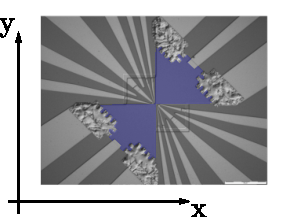
\includegraphics[width = 4 cm]{./intro/heterostructure_top_view}
			& &
			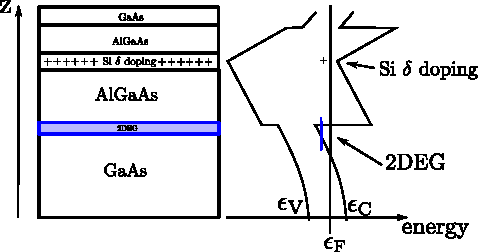
\includegraphics[width = 4 cm]{./intro/heterostructure_band_diagram} \\
			(c) & &  & \\
			& 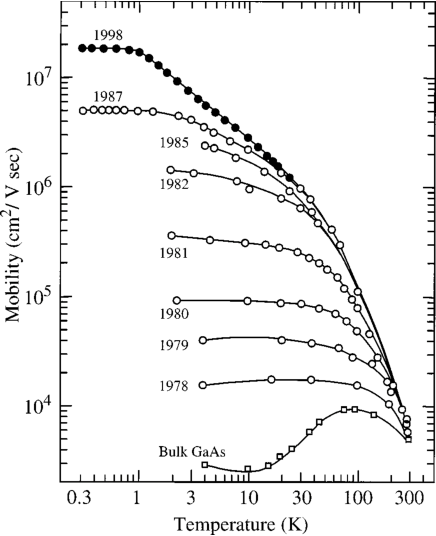
\includegraphics[width = 4 cm]{./intro/high_mobility}
			& &
			
		\end{tabular}
	\end{center}
	
	\caption{\textbf{High mobility 2D electron gas.} (a) The picture is a top view of the sample used in this manuscript where the surface colorized in blue is the 2D electron gas. (b) The schematic represents the different layers used to confine the electron gas in a two dimensional interface where the energy of the conduction band $\epsilon_{C}$ forms a quantum well as shown on the plot of energy as a function of the layer. (c) Graph from \cite{stormer1999nobel} that shown the increase of mobility in 2D electron gas with the development of the modulation doping technique based on the separation of donors and 2D electron gas in different layers of the semi-conductor heterostructure.}
	\label{fig: 2DEG}
\end{figure}

All the experiments are performed in a 2D electron gas of high mobility, the confinement of charge carriers in low dimensions allows the interaction effect.
The phenomena of integer and fractional quantum Hall effect in which the electronic transport is studied occur in two dimension, so the electrons involved in the transport are just moving in a plan.
This plan is colorized in blue in the sample picture shown in panel (a) of figure Fig.\ref{fig: 2DEG}.
These electrons are confined at an interface between two layers of semiconductors of AlGaAs and GaAs in a heterostructure, a diagram of the principal layer of the heterostructure is drawn in panel (b) of figure Fig.\ref{fig: 2DEG}.
This diagram shows in blue the plane of electrons called 2D electron gas, the modulation doping technique separates the donors which are Si atoms in a different layer than the electrons which are trapped in a quantum well between the GaAs layer of low energy conduction band and the attraction Si donors but in a AlGaAs layer of high energy conduction band.
This separation technique enables to made samples that achieve a high mobility of electrons at low temperature, the graph in panel (c) of figure Fig.\ref{fig: 2DEG}, presents the improvement other the years of the mobility of the 2D electron gas thanks to this technique, a high mobility is an other characteristic needed to observe interaction effects.


\begin{figure}[hptb]
	\begin{center}
		\begin{tabular}{c c c c}
			(a) & & (b) & \\
			& 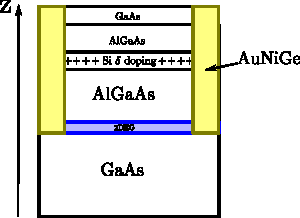
\includegraphics[width = 4 cm]{./intro/ohmic_contact_cut_view}
			& &
			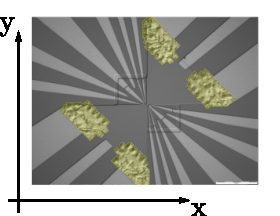
\includegraphics[width = 4 cm]{./intro/ohmic_contact_top_view} \\
		\end{tabular}
	\end{center}
	
	\caption{\textbf{Ohmic contacts that performed electrical connection with the 2D electron gas.} (a) The yellow rectangles are a schematic of the conductive alloy of AuNiGe diffused through all the layers of the heterostructure to reach the 2D electron gas. (b) The ohmics contacts on the sample top view are enhanced by a yellow false color. The size and the shape of the ohmic contacts increase the length between the electron gas and the alloy to have a better connection.}
	\label{fig: ohmic contact}
\end{figure}
 
Electrical connections with this 2D electron gas are made with different techniques, an ohmic contact is made of an alloy of AuNiGe that is diffused through the heterostructure and connects wires with the electron gas, a gate is a metallic deposit on top of the heterostructure which is capacitively coupled to the electron gas.
The electrical connections are used to manipulate the edges of the sample, indeed in the quantum Hall regime ballistic conductors appear at the edge of the sample called edge channels.
The ohmic contacts allow to directly connect the wire with the edge channels and to drive continuous current as well as high frequency current in the conductor.
This connection is made by an alloy of AuNiGe represented in the panel (a) of figure Fig.\ref{fig: ohmic contact} which is the conductive part that connect the top part of the sample with the electron gas in the heterostructure.
The top view in panel (b) of figure Fig.\ref{fig: ohmic contact} shows that the ohmic contacts are big compared to the electron gas size in order that the length of the edge of the electron gas along the ohmic contact is long enough to have a good connection with the edge channels. 
%They are also the connection used to connect a point of the edge channels to the ground.

\begin{figure}[hptb]
	\begin{center}
		\begin{tabular}{c c c c}
			(a) & & (b) & \\
			& 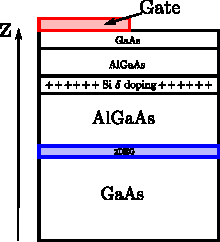
\includegraphics[width = 4 cm]{./intro/gate_cut_view}
			& &
			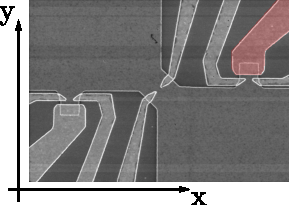
\includegraphics[width = 4 cm]{./intro/gate_top_view} \\
		\end{tabular}
	\end{center}
	
	\caption{\textbf{Gate coupled capacitively to the edge channel.} (a) The schematic shows that the gate in red is separated from the electron gas by the heterostructure, so the coupling is capacitive. (b) The gate enhanced in red is used in this manuscript to drive high frequency signal at the edge channel below.}
	\label{fig: gate}
\end{figure}

The gates can drive current in the conductor only for high frequency because they are capacitively to the edge of the electron gas and so to the edge channels.
The panel (a) of figure Fig.\ref{fig: gate} schematize the insulating layers of the heterostructure between the gate and the edge channel, and the panel (b) is a zoom on the center of the sample where the gate is enhanced in red.
In the manuscript this gate is used to add signals in the GHz frequency range to the edge channel.

\begin{figure}[hptb]
	\begin{center}
		\begin{tabular}{c c c c}
			(a) & & (b) & \\
			& 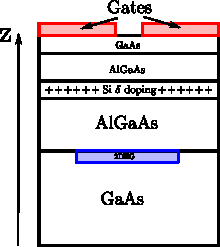
\includegraphics[width = 4 cm]{./intro/quantum_point_contact_cut_view}
			& &
			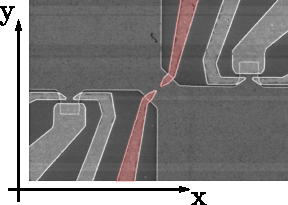
\includegraphics[width = 4 cm]{./intro/quantum_point_contact_top_view} \\
			(c) & &  & \\
			& 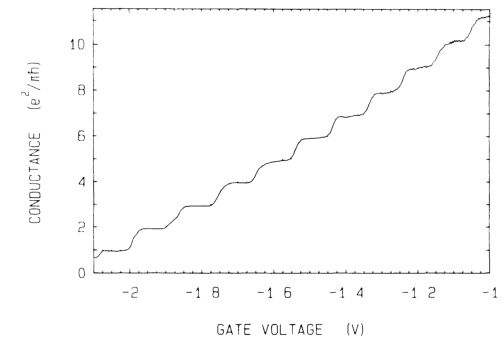
\includegraphics[width = 4 cm]{./intro/quantum_of_conductance}
			& &
			
		\end{tabular}
	\end{center}
	
	\caption{\textbf{Central quantum point used as an electronic beam-splitter.} (a) The schematic represents the electron gas in blue whose width decrease because the gates repeal the electron gas. (b) On the picture of the sample the two gates of the quantum point contact are colorized in red and are located at the narrower part of the electron gas to be able to connect or separate fully the two sides of the electron gas. (c) Graph from \cite{van1988quantized} of the conductance through a quantum point contact as a function of gate voltage. The gate voltage adjust the width of the quantum point contact which is smaller as the voltage is more negative. The conductance presents steps of twice the quantum of conductance each times two spin degenerate mode of electron can pass through the width of the quantum point contact.}
	\label{fig: qpc}
\end{figure}

They are also used with continuous voltage in the center of the sample, with a sufficiently negative voltage the gates repeal the electron gas below them, this allows controlling the geometry of the electron gas.
This control is used in the quantum point contact, this part is at the center of the sample where the electron gas is narrow and above it two gates can control its width up to the complete separation of the electron gas in two distinct parts, as one can notice on panels (a) and (b) of figure Fig.\ref{fig: qpc}.
The control of the width of the quantum point contact is used to control the transmission of electrical charges through it.
When the width of the quantum point contact is of the order of the Fermi wavelength of charges few electronic modes exist in the center of the electron gas, and by controlling the width, the gates control the number of modes and so the number of edge channels transmitted or reflected.
The conductance of the quantum point contact as a function of the voltage applied to the gates, as shown in figure Fig.\ref{fig: qpc} panel (c), is a measurement of the number of transmitted edge channels through the quantum point contact, and the curve exhibits steps of a quantum of conductance at each edge channel transmitted.
The voltage of the gates can also be set at a value between two steps of conductance, and at this voltage the last edge channel is then partially transmitted and reflected.
The quantum point contact is analogue to an electronic beam splitter for two edge channels coming from opposite sides of the quantum point contact and outgoing to two opposite edge channels with an adjustable transmission and reflection rate.

\begin{figure}[hptb]
	\begin{center}
		\begin{tabular}{c c c c}
			(a) & & (b) & \\
			& 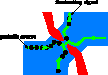
\includegraphics[height = 4 cm]{./intro/hom_shot_noise}
			& &
			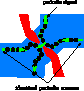
\includegraphics[height = 4 cm]{./intro/hom_noise_reduction} \\
			(c) & &  & \\
			& 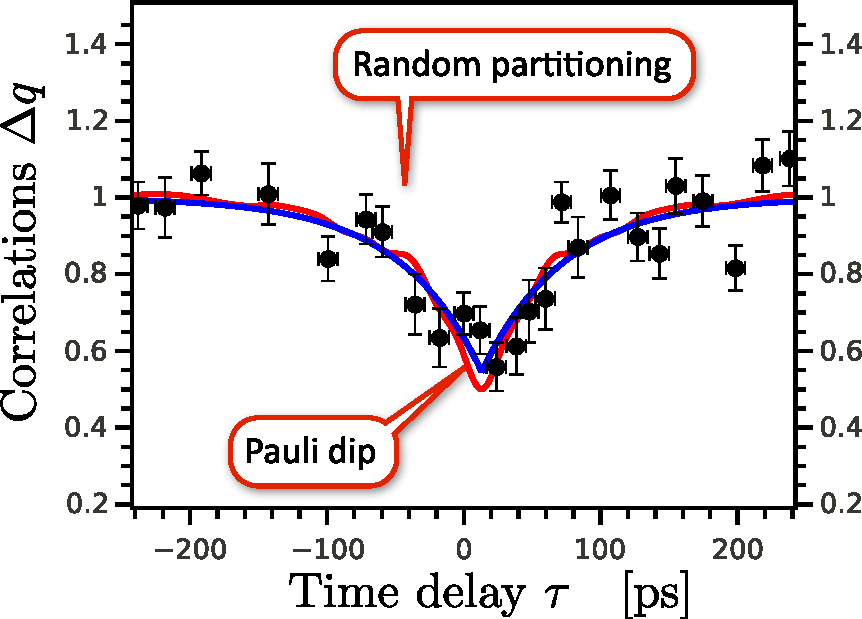
\includegraphics[width = 4 cm]{./intro/hom_measure}
			& &
			
		\end{tabular}
	\end{center}
	
	\caption{\textbf{Schematic of Hong-Ou-Mandel interferometer.} (a) In this schematic a train of periodic charges represented by black dots are emitted in a edge channel. They are randomly reflected or transmitted by the quantum point contact, so a randomly fluctuated signal called shot noise is generated in the output edge channels. (b) In this schematic two identical sources emit the same train of periodic charges. The signals in the output edge channels are not random but periodic since at each period  exactly one charge is reflected or transmitted in the output edge channels. The shot noise is suppressed, it is the Hong-Ou-Mandel interference effect. (c) Graph from \cite{bocquillon2013} where the correlation $\Delta q$ are the measured noise in one output edge channel normalised as a function of the time delay between the two sources emission. The time delay allows to control if the sources are identical or not, and the noise decrease when both sources are identical as expected with the Hong-Ou-Mandel effect.}
	\label{fig: hom}
\end{figure}

The elements of the sample used in this manuscript are one quantum point contact at the center of the electron gas, four ohmic contacts connected to the two input edge channel of the quantum point contact and to its two output edge channel, and one gate above an input edge channel.
These elements are present in the sample geometry of an electronic Hong-Ou-Mandel interferometer where two electrons sources emit a single electron at the inputs of the central quantum point contact. 
The central quantum point contact acts as a beam splitter and an incoming electron can be randomly transmitted or reflected to an output edge channel, so when electrons are periodically emitted in an incoming edge channel, they are partitioned in the two outputs channels where we get a randomly fluctuating signal called shot noise as drawn on panel (a) of figure Fig.\ref{fig: hom}.
This shot noise is suppressed when two indistinguishable electrons are emitted in the two inputs edge channel of the quantum point contact, the fermionic statistic prevent the identical electrons to exit in the same channel, this implies that there is always one electron at each output edge channel as drawn on panel (b) of figure Fig.\ref{fig: hom}.
The measurement of the shot noise in an output channel gives information about the overlap of the two electronic states in the input edge channels, the experience demonstrating this electronic Hong-Ou-Mandel effect has been realized in \cite{bocquillon2013} and the main measurement is plotted on panel (c) of figure Fig.\ref{fig: hom} and used to study decoherence and fractionalization of single electron emission \cite{marguerite2016decoherence}.
The measurement of noise will be used in the three chapters of this manuscript to deduce information on the electronic states.
